\documentclass[a4paper,10pt]{article}
\usepackage[utf8x]{inputenc}
\usepackage{array}
\usepackage{graphicx}
\usepackage{float}
\usepackage{color}
\usepackage{alltt}
\usepackage[T1]{fontenc}
\usepackage{ae,aecompl}

%opening
\title{Context Free General Top Down Parsing in Cubic Time}
\author{Arnold Lankamp}

\begin{document}

\maketitle

\begin{abstract}

In this article we will describe our general top-down parsing algorithm. The intent of this algorithm is to be both easy to comprehend and able to perform well for any grammar. In our opinion users should not be required to refactor their grammars to enable the parser to complete within an acceptable amount of time. Nor should it be difficult to comprehend what is going on under the hood, enabling one to easily visualize what is going on. From a developer's point of view, creating an implementation of the algorithm should also be similarly easy to do; often this is something that requires a considerable amount of effort to get right.

It sounds fairly ambitious, but we managed it. We created a general parsing algorithm that is both easy to understand and can compete with any other general parsing algorithm out there in terms of scalability and performance.

\end{abstract}

\section{Introduction}

For our parsing algorithm we choose for a top-down approach, as it is more in-line with human thinking then bottom-up. This makes both the algorithm and implementation(s) easier to comprehend and makes parse traces easier to visualize. Top-down parsers also have no need for complicated parse tables; the translation from a grammar to a for the parser usable format can simply be one-on-one, without any additional trickery or risks of parse table explosion. Lastly, top-down parsers can also generate understandable error reports more easily, which is a very welcome feature. We call our parser, the Scannerless General Top Down Binary Forest Parser or SGTDBF.

To give an impression of the capabilities of our algorithm and implementation, we will enumerate some highlights first:
\begin{itemize}
 \setlength{\itemsep}{0pt}
 \setlength{\parskip}{0pt}
 \setlength{\parsep}{0pt}
 
 \item Worst-case cubic space and time bounds with respect to the length of the input.
 \item Linear performance on unambiguous grammars.
 \item Deterministic on all types of LL and LR grammars.
 \item No penalty for handling nullables, hidden recursive or otherwise.
 \item No penalty for being scannerless.
 \item Generating or hand crafting the parse table / code from a grammar is trivial.
 \item Parse traces are easy to visualize.
\end{itemize}

\section{Recognizer}

First we will discuss the algorithm for the recognizer, for simplicity's sake. Further on in this article we will explain how the recognizer can be extended to become a parser.

\subsection{Graph}

To represent the parallel stacks we use a directed cyclic graph; inspired by GLR's Graph Structured Stack. While it serves a similar purpose, the way it is used is completely different. Simply put, while GLR parsers store their `history' in the GSS, we use it to model possible `futures'.

In our case we assign a unique identifier for every item in the grammar. For example; if we take the following grammar: $S\,::=\,AB\,|\,BA,\,A\,::=\,a,\,B\,::=\,b$, we would assign these identifiers as follows: $.S$(-1), $.AB$(0), $A.B$(1), $.BA$(2), $B.A$(3), $.a$(4) and $.b$(5). These identifiers are needed to be able to handle the sharing of graph nodes correctly, so regardless whether or not comparable items exist, they should not be merged. Each graph node consists of an item, edges back to their `parents' in the graph, information about its `right neighbour' in the production and the location in the input string it is associated with. Each stack node is unique for each identifier, location combination.

\subsection{The basic principle}

The basic idea behind the algorithm is fairly straightforward. In general terms this is how it works:

\begin{enumerate}
 \setlength{\itemsep}{0pt}
 \setlength{\parskip}{0pt}
 \setlength{\parsep}{0pt}

 \item Expand the left most node of every production that did not match anything yet on all stacks, until no stacks can be expanded anymore (i.e. they all have a terminal at the bottom).
 \item Match all nodes on the bottom of the stacks to the input. Reduce the ones that match, remove the ones that do not.
 \item Reduce the nodes on all stacks that matched something and have them queue the `next' node in the production they are part of where applicable, until no reductions are possible anymore.
 \item If there are nodes queued for expansion go to 1.
 \item If the end of the input has been reached and we have at least one derivation for one of the start symbols, we are successful; otherwise recognition failed.
\end{enumerate}

\pagebreak
\subsection{Pseudocode}

In this section we will present and discuss the pseudocode of the recognizer. Note however that this pseudocode already contains the edge related optimizations listed in section \ref{sec:edgeOptimizations}. This was done since, besides improving performance, they simplify the implementation of the algorithm slightly and they enable the recognizer to achieve most of its advertised performance guarantees. We will not go into detail about how these optimization work or why they are correct here; please refer to the indicated section for more details. Other optimizations were not merged in with the code presented here, since they either complicate things too much or can be implemented in multiple ways; a decision we would like to leave for the implementor. For the same reason, the hidden right recursion fix, discussed in section \ref{subsec:hiddenRightRecursion}, was left out here as well. On the other hand, the nullable fix described in section \ref{subsec:nullables} is present.

\subsubsection{Main}
{\small
\begin{verbatim}
main(){
  toExpandSet.add('startNode');
  expand();
  
  while(hasMoreStacksToReduce(toReduceStore)){
    expandedSet.clear();
    reducedStore.clear();
    sharedNextSet.clear();
    toReduceSet = getStacksToReduce(toReduceStore);
    
    do{
       reduce();
       expand();
    }while(isNotEmpty(toReduceSet));
  }
  
  if(endOfInputHasNotBeenReached()) error;
}
\end{verbatim}
}

This is the main function of the recognizer. It starts with building the stacks for the first level, by queueing the `start node' and expanding it. Once it has done so it will keep alternating between reducing and expanding until there are no more stacks left alive. At the start of each iteration we get the appropriate {\bf toReduceSet} from the {\bf toReduceStore}. The {\bf toReduceStore} is a collection that contains one {\bf toReduceSet} for each level. At the end of each iteration we check whether or not we need another iteration in the current level or need to shift to the next one. In case we shifted we need to discard all level specific data. This behaviour is necessary to be able to handle nullables properly. For more information about the handling of nullables see section \ref{subsec:nullables}.

Note that the {\bf toReduceStore} needs to be implemented as an array or table with O(1) look-up time; otherwise it is not possible to guarantee worst-case cubic time complexity.

Also note that after each iteration all graph nodes that are no longer reachable through any of the nodes in the {\bf toReduceStore}, can be discarded.

\pagebreak
\subsubsection{Expansion}
\label{subsec:pseudocodeExpand}
{\small
\begin{verbatim}
expand(){
  while(node <- toExpandSet){
    if(node.isTerminalOrEpsilon()){
      if(node.match(input)){
        toReduceStore.add(node);
      }
    }else{
      if(cachedEdges.contains(node.sort)){
        edgesSet = cachedEdgesMap.get(node.sort);
      }else{
        edgesSet = createAndCacheEdgesSet(node.sort);
        
        for(childNode <- getAlternatives(node)){
          childNode = childNode.initialize(location);
          childNode.setEdgesSet(edgesSet);
          toExpandSet.add(childNode);
        }
      }
      edgesSet.addEdge(node);
      
      if(reducedStore.contains(node.sort)){
        toReduceSet.add(node);
      }
    }
  }
}
\end{verbatim}
}

This is the expand loop. It will iterate over the {\bf toExpandSet} until there are no more stacks queued for expansion. While expanding we check the type of the node we are handling. If the node is a terminal or an epsilon it needs to match the input (epsilons naturally always match). If it matches, it is added to appropriate {\bf toReduceSet} in the {\bf toReduceStore}; otherwise we discard it, causing the stack it was associated with to die of. If the node is a non-terminal, we check if there is a cached set of edges available for that non-terminal sort. If there is, we queued the alternatives for that non-terminal sort before; since this is the case, we merge the current stack with the already expanded ones by adding an edge to the cached {\bf edgesSet} for this non-terminal sort. If a cached {\bf edgesSet} is not available, we have not encountered a non-terminal of this sort yet and need to expand it. We do this by retrieving its alternatives and queueing the first `child' of each alternative for expansion, by adding them to the {\bf toExpandSet}. We also create and cache a set of edges for this non-terminal sort, to which an edge to the current node will be added. Each of the `child' nodes will receive a reference to this {\bf edgesSet}, which may be updated with additional edges later on in the expansion process.

Finally we check whether or not there have been nullable reductions for the non-terminal sort associated with the current node. This can occur because we to multiple iterations in this same level to be able to handle nullables properly. If such a nullable reduction is present in the {\bf reducedStore}, we queue the current node for reduction by adding it to the {\bf toReduceSet} for the current level. We will discuss the handling of nullables in more detail in section \ref{subsec:nullables}.

\pagebreak
\subsubsection{Reduction and moving}
{\small
\begin{verbatim}
reduceOrMove(){
  while(node <- toReduceSet){
    if(node.lastInProduction()){
      for(edgeLevel <- node.edgesPerLevel){
        sort = edgeLevel.getOne().sort;
        if(reducedStore.notContains(sort)){
          reducedStore.add(sort);
          
          for(edges <- edgeLevel){
            toReduceSet.add(parent);
          }
        }
      }
    }else if(node.hasNext()){
      next = node.next.initialize(location);
      
      if(sharedNextSet.contains(next)){ // Sharing
        next = sharedNextSet.get(next);
      }else{
        sharedNextSet.add(next);
        toExpandSet.add(next);
      }
      next.addEdges(node.edges);
    }
  }
}
\end{verbatim}
}

This is the reduce or move loop. It will iterate over the {\bf toReduceSet} until there are no more stack nodes queued for reduction. When a node is being reduced, one of two things can happen. Either it is the last node in the production and we need to queue the `parents' of this node for reduction (if not reduced of queued for reduction already), by adding them to the {\bf toReduceSet}. Otherwise we need to move to the `next' node in the production, queue this `next' node for expansion and transfer all edges from this node to it. If the `next' node has already been scheduled for expansion it will be present in the {\bf sharedNextSet}. If this is the case we need to retrieve the shared equivalent of this `next' node from this set and add the edges to that node instead.

The edges are grouped by level. This level indicates the start location of the node the edge points to. To check whether or not the parents of a node need to be queued for reduction, we get one of the edges from each {\bf edgeLevel} and check if there are reductions for the non-terminal sort associated with the node this edge points to, by consulting the {\bf reducedStore}. If a node has not been reduced yet, we queue all of the nodes that are pointed to from edges in that {\bf edgeLevel} for reduction; otherwise we do not. This will work correctly since every node containing a non-terminal of the same sort always has exactly the same alternatives in the same level. Note that this behaviour is not a necessity, but an optimization (which reduces the number of edge visits by a factor between one and the number of non-terminals in the grammar). For more information about this optimization see section \ref{subsec:edgeVisitOptimization}.

The {\bf reducedStore} is a dual layered data structure. The first layer is indexed by the {\bf start location} of the node and the second layer by the sort of the non-terminal in the node. For each level the {\bf reducedStore} can contain a variant for every non-terminal for each possible substring up until the current location. This {\bf reducedStore} is necessary to keep track of which nodes have or have not been reduced yet. The first layer of the {\bf reducedStore} needs to be implemented as an array or table with O(1) look-up time; otherwise it is not possible to guarantee worst-case cubic time complexity.

\subsection{Correctness}

In this section we will go into detail on some special cases that deserve some additional explaination.

\subsubsection{Left recursion}
First of all, left recursion. Normal top-down parsers cannot handle grammars containing left recursion, since they keep expanding left recursive rules indefinitely, preventing implementations of these kind algorithms from terminating. Because we introduce sharing into the graph, which leads to automatic terminalization of all these rules, this undesirable behaviour is prevented from manifesting. By terminalization we mean that the expansion phase converges to a point at which each stack has a terminal at the bottom and thus cannot be expanded further. For example, if we take the grammar:\\
$S ::= A$\\
$A ::= Aa\,|\,a$\\
We would expand these rules in the following way:
\begin{figure}[H]
\centering
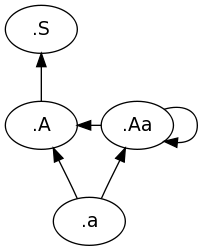
\includegraphics[scale=0.5]{left-recursive.png}
\caption{Graph representation of an expanded left-recursive grammar.}
\end{figure}
As can be seen a cycle is added to the graph, since $.Aa$ is, in a way, a child of itself. To see how left recursive grammars work in action see section \ref{sec:tracesLeftRecusive}.

\subsubsection{Cycles}
Cycles present another issue that needs to be handled. Similarly to left recursion, this problem is automatically resolved by the sharing that is introduced into the graph. Instead of infinitely expanding the circularly dependent production rules, a cycle will be added to the graph, halting the expansion process for the involved rule. The reduction process will also terminate, since it will only perform the reductions for each node once.

\subsubsection{Nullables}
\label{subsec:nullables}
Nullables also deserve some attention. Nullables do not pose any difficulties in most cases; however when a production contains two or more consecutive nullables, hidden left- / right-recursive or otherwise, problems arrise. The first of these problems is sharing related.

We will describe the issue by illustrating what would happen in a version of the implementation of the algorithm which does not contain the fix.
Consider the following grammar:\\
$S ::= AA$\\
$A ::= C$\\
$C ::= \epsilon$\\
Input = <empty>\\
After the first expansion and reduction phase, we matched both $.C$ and the $.AA$ at location $0$. Next we move to $A.A$; when we expand $A.A$ node we notice $.C$ has already been expanded at the current level ($0$), causing recognition to stop. Since there is no work left to do the recognizer will terminate with an error, as we failed to produce any derivations for the input string.

In our algorithm we address this issue by checking whether or not the non-terminal sort associated with the node we are currently attempting to expand has nullable results in the current level. If this is the case we queue this node for reduction. Additionally, we also update the appropriate set of edges (as described in section \ref{subsec:pseudocodeExpand}). This is necessary, since the children of the current node were already expanded in a previous iteration in the same level; this means the current stack needs to merge with the stacks of these children, so no future (non-nullable) reductions involving these children will go missing. We will keep alternating between expansion and reduction until no more work can be done for the current level (i.e. there are no more nullable reductions); once this is the case, we shift to the next level.

\subsubsection{Hidden right recursion}
\label{subsec:hiddenRightRecursion}
Unfortunately this only solves one of the two nullable related problems. The other issue that needs to be resolved is related to hidden right recursion.

Consider the following grammar:\\
$S\,::=\,SS\,|\,a\,|\,\epsilon$\\
Input = $a$\\
Imagine we matched the first part of the tree and are at level $1$ now. We are trying to recognize $.SS$ and $S.S$, where $S.S$ has a prefix that starts at $0$. This means $.SS$ only has edges that point to nodes in level $1$ and $S.S$ only has edges that point to nodes in level $0$. The problem is that the order in which we handle these two nodes will determine whether or not we recognize all derivations. If we would move from $S.S$ to $SS.$ first, $SS.$ will only have edges to level $0$ associated with it, so this will cause us to miss the reductions to level $1$ when $SS.$ is handled. This happens because the stack merge at $S.S$ took place after $S.S$ is handled, preventing the edges present on $.SS$ from being transfered, through $S.S$, to $SS.$. On the other hand, if we would move from $.SS$ to $S.S$ first, the stacks would merge before $S.S$ is handled. In this case $S.S$ would contain edges to both the nodes in level $0$ as the ones in $1$ before we move to $SS.$, which does lead to a correct result.

This order dependency is something we cannot enforce, so we need another solution for this problem. We solved this by propagating edges forward through the production, when necessary. If we are currently handling a node associated with nullable derivations and are moving to the next node in the production, we need to check whether or not this next node is handled yet and if it is associated with nullable derivations as well. If this next node is both handled and has nullable derivations associated with it, we tranfer all edges that are absent on this next node to it. If missing edges were transferred, we need to continue the propagation of these transferred edges to the node beyond this next node and so on until the last node in the production is reached. For each edge that is transferred to the last node in the production a reduction needs to be performed. This way we can be sure all derivations will be traversed.

Also note that, since this propagation only happens within a single level and does not introduce any real extra work, it does not influence worst-case behaviour. This is because all stack merges would have happened regardless of their timing; the only difference is that the exact same amount of work they normally generate gets distributed over multiple visits of the same node. Consequently, the performance impact of this solution is very low in general; close to non-existent even, since it only requires one cheap constant time check on each node visit.

\subsubsection{Termination}
Another questions that some people will have on their mind is: ``does it terminate?". Ofcourse it does. The reason for this fairly obvious and can be even explained in one sentence; since we move forward to the next level once all work is done in the current level and we share all graph nodes within each level (of which there are a finite amount), causing the expansion and reduction phases to converge to a point where no more work can be done in a level, we are always able to reach the end of the input string (assuming the input string has a finite length), completing recognition.

\subsubsection{Breadth-first vs depth-first}
\label{subsec:breadthFirstVsDepthFirst}
Another requirement of the algorithm, of which the reason may not be immediately obvious, is that it needs to be level synchronized. We will demonstrate why the depth-first sibling does not work correctly without modification and why this modification would break the cubic time bound, by means of an example. Consider the following grammar: $S ::= SSS\,|\,a\,|\,aa$. Now imagine we are somewhere in the middle of recognizing an input string containing a number of $a$'s; currently we are recognizing $SS.S$, which matches with one $a$. The preceding items that belong to this production, $.SSS$ and $S.SS$ both recognized one $a$ as well. Causing $S(S(a),S(a),S(a))$ to be reduced at this location. We progress a bit more and are now recognizing $.SSS$ at a location that is one character earlier in the input string as the other $.SSS$ we recognized before; this time it matches $aa$. Since we now end up at a $S.SS$ node at a location where it was already recognized, we do not progress further; this node needs to be shared, otherwise we would do duplicate work, breaking the cubic time bound. However, in the scheme we are using, sharing this node means we stop recognizing the current derivation, preventing reductions from being executed. Which in this case will mean that we fail to recognize the derivation $S(S(aa),S(a),S(a))$ at the current location. If we would be using a different grammar it could even cause recognition to fail entirely because of this behaviour.

This problem could be solved by tracing forward through the production, gathering any potential missing derivations and executing reductions where necessary; similarly to how we solved the hidden right recursion issue. However, counterary to the hidden right recursion solution, which is limited to a single level and consequently not bound to the length of the input, we would potentially need to trace all possible continuations of a production to the end of the input string upon every stack merge. This would cause the algortihm to become unbound polynomial in time, since it would lead us to visit nodes $O(N^P)$ times in the worst-case (where $N$ is the length of the input string and $P$ is the length of the longest production).

In our opinion the solution for this problem is both to complicated and, above all, unnecessary. Since our algorithm is breadth-first, we will never have (non-nullable) stacks running ahead of others, eliminating the possibility of this behaviour popping-up.

\subsection{From grammar to recognizer}

Converting a grammar to a recognizer or parser, either by hand writing or generating it, is relatively straight forward. All that is needed is a direct translation from the grammar rules to either functions or a table like data structure. Basically the recognizer just needs to know what alternatives are associated with each left-hand-side. In case we are generating code, this would mean that we need one function per non-terminal sort, which contains logic that informs the recognizer about what alternatives should be expected.

Since the mapping between the original grammar and the code or table is one-on-one, it is possible to implement or edit it by hand without much effort. In fact handcrafting it is about as simple as writing the grammar itself (although more cumbersome).

Another advantage is that, in combination with the top-down-ness of our algorithm, it makes tracing errors in a grammar easier; if you would like to know why something does not match at a certain position, you can just go through it with a debugger to see what happens. Your degree of success naturally depends on the amount of stacks that are alive at the moment you are trying to observe, which is linked to the amount of non-determinism in the grammar, but at least the possibility to do so exists.

\subsection{Example traces}

To illustrate how the recognizer works in action, we constructed some example traces using various grammars to give an impression.

\pagebreak
\subsubsection{Straight forward}
First we will take a look at a simple non-ambiguous grammar:\\
$S ::= AB$\\
$A ::= a$\\
$B ::= b$\\
Input = $ab$

\begin{enumerate}
 \setlength{\itemsep}{0pt}
 \setlength{\parskip}{0pt}
 \setlength{\parsep}{0pt}
 
 \item expand $.S$
 \item expect $.AB$
 \item expand $.AB$
 \item expect $.a$; $.a$ matches
 \item reduce $a.$ and follow edge to $.AB$
 \item move from $.AB$ to $A.B$
 \item expand $A.B$
 \item expect $.b$, $.b$ matches
 \item reduce $b.$ follow edge to $A.B$
 \item reduce $AB.$ and follow edge to $.S$
 \item parse for $S.$ is complete 
\end{enumerate}
This one is easy to follow and does not really need any additional explanation.

\subsubsection{Left recursive}
\label{sec:tracesLeftRecusive}
Next up is a grammar containing a left-recursive rule:\\
$S ::= A$\\
$A ::= Aa\,|\,a$\\
Input = $aaa$

\begin{enumerate}
 \setlength{\itemsep}{0pt}
 \setlength{\parskip}{0pt}
 \setlength{\parsep}{0pt}
 
 \item expand $.S$
 \item expect $.A$
 \item expand $.A$
 \item expect $.Aa$ and $.a$; $.a$ matches
 \item expand $.A$ $\Rightarrow$ $.A$ shared
 \item reduce $a.$ and follow edges to $.A$ and $.Aa$
 \item reduce $A.$ and follow edges to $.S$
 \item parse for $S.$ is incomplete and is discarded
 \item move from $.Aa$ to $A.a$; $A.a$ matches
 \item reduce $Aa.$ and follow edges to $.A$ and $.Aa$
 \item reduce $A.$ and follow edges to $.S$
 \item parse for $S.$ is incomplete and is discarded
 \item move from $.Aa$ to $A.a$; $A.a$ matches
 \item reduce $Aa.$ and follow edges to $.A$ and $.Aa$
 \item reduce $A.$ and follow edges to $.S$
 \item parse for $S.$ is complete
 \item move from $.Aa$ to $A.a$; $A.a$ does not match since the EOI has already been reached
\end{enumerate}
As one can see, when expanding $.A$ for the second time (at 5), sharing is detected causing a cycle to be added to the graph. Reductions of $Aa.$ follow the edge back to $.Aa$ which will move to $A.a$; this will lead to one $a$ being matched at each `iteration' and ultimately consuming all of them.

\subsection{Worst-case time complexity}
\label{subsec:recognizerComplexity}

We are designing a parsing algorithm that is intented to scale as well as is possible, regardless of the input grammar. For this reason, the recognizer must not break the cubic time bound. Here we will prove that we remain within this bound.

Since the graph only contains nodes that we expect to `encounter', there are at most $O(N)$ of them; where $N$ is the number of characters in the input string. Each node only has one edge to each of its possible parents per level and there are $N$ levels, so there are at most $O(N)$ edges per node. In the worst-case there are $N$ times $O(N)$ nodes that match a substring that ends at the `current' level. When moving to the `next' node in the production, all edges of these nodes need to be carried over. Since these sets of edges need to be merged, the time this operation needs to complete is equal to the number of levels before (and including) the `current' level (so $N$ at most). So this operation will execute in $O(N^3)$ time at most in the worst-case.

Reducing consumes $O(N^3)$ time in the worst-case as well. Every edge is associated with one reduction per level per graph node at most. Each of these edges can be associated with $O(N)$ nodes per level; one per level before the current level. There are $N$ levels, so each edge will be visited $O(N^2)$ times. Since there are never more then $O(N)$ edges in total, we can conclude that the number of visited edges falls within the $O(N^3)$ bound. Each of the operations executed during an edge visit completes in constant time, so the worst-case time bound of the reducer is directly related to the number of edge visits.

Overall, this means that the algorithm remains within cubic time bounds in worst-case scenarios.

\subsection{Unambiguous case time complexity}
\label{subsec:unambiguousTimeComplexity}

Keeping worst-case behaviour in check is great, but is generally of lesser importance then having good performance and scalability in the more common cases. Here we will prove that our algorithm is linear, not only for deterministic (such as LL and LR) grammars, but for all unambiguous context-free grammars.

The reason for this is fairly simple. In our algorithm a stack merge or edge that is visited twice only occurs in cases where an ambiguity is encountered. The cause of these events is always that a certain portion of the input string can be derived in more then one way. When parsing an input string for an unambiguous language neither of these events can ever occur. The result of this is that every graph node can only have one edge and one unique graph node that preceded it. While the stack can split, this will never result in more then one node per non-terminal sort per level. Combined with the linear time graph expansion guarantee, due to the optimization discussed in section \ref{subsec:nodeExpansionOptimization}, this means we can recognize every possible input string for an unambiguous grammar in $O(N)$ time.

Note however that, while we can recognize input for unambiguous grammars in linear time, performance will degrade by a factor that is relative to the amount of non-determinism in the grammar. Additionally, performance degradation for ambiguous grammars is also fairly graceful. Meaning that input strings for near unambiguous grammars will also be parsed in near linear time.

\pagebreak
\subsection{Error reporting}

Finally we would also like to note the relative ease with which understandable error reports can be generated. When a parse error is encountered it is trivial to generate all possible traces back to the root from the current level, since we have all the necessary information present in the graph. In these traces a user can exactly see where recognition failed, but also what did match up until this point.

\section{Parser}

\subsection{Parse forest}

To represent the parse forest we use a format that was especially designed for this parser, to ensure worst-case behaviour remains within cubic space and time bounds. We call it `deflattenized', for lack of a better description. While its purpose is similar to binarized SPPFs, its implementation is somewhat different.

The parse forest consists of nodes. Every node in the forest contains a result and a set of prefixes. Each result represents a substring for a certain symbol. In case this symbol is a non-terminal, this result contains one or more references to alternative representations of the substring it denotes. If the symbol is a terminal, it will just represent that specific terminal. The set of prefixes contained in the node hold all possible alternatives for the preceding item in the production. (Naturally this set is empty for the node associated with the first item in the production). A prefix only consists of a reference to a node. If one traces all possible paths through this representation of a production to the start, one will get all alternatives for this production of the substring it represents.

Note however that there is a strong relation between the internal graph representation of the parser and the resulting parse forest. Because of this relation, the resulting parse forest can contain cycles.

Another thing worth mentioning is that it is not strictly required to use a binarized parse forest in combination with our parser. In reality any kind of representation could be used, though it is highly recommended to use the one described here for optimal performance and ease of implementation. For more information about the cubic vs non-cubic parse forest tradeoff see section \ref{subsec:Flattening}.

\pagebreak
\subsubsection{Example}
To give an idea of what a typical parse forest would look like we will give a simple example using the following grammar:\\
$S\,::=\,AAA$\\
$A\,::=\,a\,|\,aa$\\
Input = $aaaa$

\begin{figure}[H]
\centering
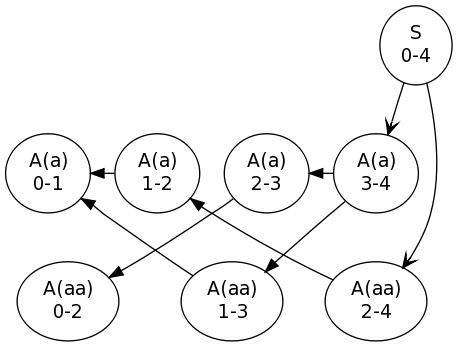
\includegraphics[width=0.5\textwidth]{a_aa-forest.png}
\caption{A visual representation of the parse forest, showing all derivations for the given input string. The numbers indicate the start and end position of the matched substring.}
\end{figure}

In the figure above we see the parse forest. It illustrates how the parse results are stored in memory.

To show how we can obtain all possible derivations from this parse forest, we will list them in the table below; which relates each path through the forest to a derivation.

\begin{table}[H]
\centering
\begin{tabular}{ p{15em} p{15em} }
Derivation & Forest path\\
\hline
S(A(a),A(a),A(aa)) & $A0$-$1$ $\leftarrow$ $A1$-$2$ $\leftarrow$ $A2$-$4$\\
S(A(a),A(aa),A(a)) & $A0$-$1$ $\leftarrow$ $A1$-$3$ $\leftarrow$ $A3$-$4$\\
S(A(aa),A(a),A(a)) & $A0$-$2$ $\leftarrow$ $A2$-$3$ $\leftarrow$ $A3$-$4$
\end{tabular}
\caption{A flattened representation of the parse forest, listing all derivations.}
\end{table}

\pagebreak
\subsection{Pseudocode}

Augmenting our recognizer with parse tree construction code is trivial. Only a few minor adjustments are needed. Relevant pieces of code, containing changes or additions, are highlighted in italic.

\subsubsection{Main}
{\small
\begin{alltt}
main()\{
  toExpandSet.add('startNode');
  expand();
  
  while(hasMoreStacksToReduce())\{
    expandedSet.clear();
    resultStore.clear();
    sharedNextSet.clear();
    toReduceSet = getStacksToReduce();
    
    do\{
       reduce();
       expand();
    \}while(isNotEmpty(toReduceSet));
  \}
  
  if(endOfInputHasNotBeenReached()) error;
  \textit{
  return resultStore.get('startNode');}
\}
\end{alltt}
}

The only things that need to be changed in the main function to transform the recognizer into a parser are the returning of the final result (if not in error) and replacing the {\bf reducedStore} by {\bf resultStore}. The {\bf resultStore} is similar to the {\bf reducedStore}, except that it also contains the result associated with the non-terminal sorts in the store.

Note that, like the {\bf reducedStore}, the {\bf resultStore} is a dual layered data structure. The first layer is indexed by the {\bf start location} of the result and the second layer by the sort of a non-terminal. In each level the {\bf resultStore} can contain a variant for every non-terminal for each possible substring up until the current location. The first layer of the {\bf resultStore} needs to be implemented as an array or table with O(1) look-up time; otherwise it is not possible to guarantee worst-case cubic time complexity.

\pagebreak
\subsubsection{Expansion}
{\small
\begin{alltt}
expand()\{
  while(node <- toExpandSet)\{
    if(node.isTerminalOrEpsilon())\{
      if(node.match(input))\{
        toReduceStore.add(node);
      \}
    \}else\{
      if(cachedEdges.contains(node.sort))\{
        edgesSet = cachedEdgesMap.get(node.sort);
      \}else\{
        edgesSet = createAndCacheEdgesSet(node.sort);
        
        for(childNode <- getAlternatives(node))\{
          childNode = childNode.initialize(location);
          childNode.setEdgesSet(edgesSet);
          toExpandSet.add(childNode);
        \}
      \}
      edgesSet.addEdge(node);
      \textit{
      if(resultStore.contains(node.sort))\{}
        toReduceSet.add(node);
      \}
    \}
  \}
\}
\end{alltt}
}

The expansion code does not need to change a lot, since it has limited interation with parse results. The only change is related to the {\bf reducedStore}, which has been replaced by the {\bf resultStore}. In this context the {\bf resultStore} serves a similar function as the {\bf reducedStore} in the recognizer; to check whether or not there are nullable reductions available for a certain non-terminal sort. We will discuss the {\bf resultStore} in more detail further on in this section.

\pagebreak
\subsubsection{Reduction and moving}
{\small
\begin{alltt}
reduceOrMove()\{
  while(node <- toReduceSet)\{
    if(node.lastInProduction())\{
      for(edgesLevel <- node.edgesPerLevel)\{\textit{
        if(resultStore.contains(edgesLevel.getOne().sort))\{
          result = resultStore.get(edgesLevel.getOne().sort);
        \}else\{
          result = createResult(edgesLevel.getOne());}
          for(edges <- edgesLevel)\{
            toReduceSet.add(parent);
          \}
        \}\textit{
        result.addAlternative(node.prefixes, node.results);}
      \}
    \}else if(node.hasNext())\{
      next = node.next.initialize(location);
      
      if(sharedNextSet.contains(next))\{ // Sharing
        next = sharedNextSet.get(next);
      \}else\{
        sharedNextSet.add(next);
        toExpandSet.add(next);
      \}
      next.addEdges(node.edges);\textit{
      next.updatePrefixes(node.prefixes, resultStore.get(node));}
    \}
  \}
\}
\end{alltt}
}

The reduce or move code need to be modified more extensively. Basically two things need to be added.

First of all the storing of results. We need to create (at most) one {\bf result} per sort of non-terminal for each matched substring; no more then that. In the recognizer code we used the {\bf reducedStore} for a similar purpose. Here it is replaced by the {\bf resultStore}, which basically is the same thing, but with results associated with the non-terminal sorts in the store.

Secondly we need to add {\bf prefixes} to the nodes that are being queued for expansion when we are moving to the {\bf next} node in the production. We do this by creating a new prefix using the prefix of the current node and its result and adding it to the {\bf next} node. We add the prefixes to graph nodes for convenience reasons; regardless of where the result(s) of the node end, they will always share the same prefix. By adding the prefixes to the graph nodes they are easy to retrieve; all these nodes need is a collection that holds all the prefixes for it, grouped by the start location of the production each induvidual node is a part of.

\pagebreak
\subsubsection{Results}
{\small
\begin{alltt}
\textit{createResult(node)\{
  result = allocateResult(node.startLocation, node.sort);
  resultStore.add(result);
  return result;
\}}
\end{alltt}
}

We also need a function for creating {\bf results}. Every time a result is created we need to add it to the {\bf resultStore}. The {\bf start position} and non-terminal {\bf sort} of the given node are used as keys. Like the {\bf reducedStore} the {\bf resultStore} is a dual layered datastructure, where the first layer is indexed using the {\bf start position} of the node and the second layer by the non-terminal {\bf sort} the node represents.

\subsection{Correctness}
\label{sec:parserCorrectness}

Since the conversion of our recognizer to a parser is so trivial, the parser is as correct as the recognizer. The only thing that may require some additional explaination, is the handling of hidden right recursion.

\subsubsection{Hidden right recursion}
As mentioned before hidden right recursion needs some extra attention. However since the recognizer produces all derivations we do not run into any real issues here. We just need to ensure we also properly propagate the prefixes along with the edges, as discussed in section \ref{subsec:hiddenRightRecursion}. Note that special care needs to be taken by the implementor to prevent equal prefixes from being added more then once.

One way to solve this is by marking each set of prefixes associated with a certain start location in a graph node with one bit that indicates whether or not a prefix of which the last result node is nullable was added to this set yet, either by a `move' or by propagation. Before adding a prefix to one of these prefix sets, we check whether or not this bit is set; if it is, we do not add the prefix, since it will already be present in the set. We know this, because every prefix is unique for every combination of its start location and the start location of the last result node in the prefix. Since the last result node of the prefix is always nullable in the case we want to verify, its unicity can be determined by the start location alone. This is why checking this one bit is sufficient to determine whether an identical prefix is already present or not.

\subsection{Worst-case complexity}

We looked at the worst-case behaviour of the recognizer in section \ref{subsec:recognizerComplexity} and proved that is does not break the cubic time bound. For the parser to be able to make the same guarantee, the size of the parse forest must be, at most, cubic in the length of the input. The reason for this, is that it is impossible to construct a greater then cubic parse forest in a cubic amount of time. Here we will prove that we do not break this space bound.

Every node in the tree is identified by the substring its contained result represents and its prefixes. There can be only one result per substring, this means there are at most $O(N^2)$ results. The prefix sets are identified by the start and end position of the substring they represent, so there are at most $O(N^2)$ of them. Each prefix set can contain up to $N$ different prefixes, which all denote the same substring; at most one per location (before the current location) in the input string. So there are at most $O(N^3)$ prefixes. The number of unique nodes is determined by multiplying the number of results by the number of prefix sets. However, since a prefix set can only be matched in a node, together with a result that starts at the same position as the prefix ends each prefix set can be associated with $O(N)$ different results at most. Hence the number of unique nodes is limited to $O(N^3)$, making the parse forest $O(N^3)$ worst-case. Note that all prefix sets can be shared regardless of the end position of the node they are matched to; this has no effect on worst-case behaviour, but does improve performance and decreases memory usage.

\subsection{Unambiguous case complexity}

The scalability guarantees made for the recognizer do not change when it is extended to a parser. The reason for this is that each additional operation the parser requires over the recognizer, can be implemented in a way that only imposes a constant amount of extra work.

\subsubsection{Worst-case statistics}
In this section we will highlight the $O(N^3)$ behaviour of the recognizer / parser in worst-case scenarios. To accomplish this we will give an overview of the most relevant parser statistics for the following grammar:\\
$S\,::=\,SSS\,|\,SS\,|\,a$\\
Input = $a * 2$ to $a * 10$, $a * 50$, $a * 100$, $a * 200$, $a * 300$, $a * 400$ and $a * 500$

\begin{table}[H]
\centering
\begin{tabular}{ | p{7ex} | p{7ex} | p{7ex} | p{10ex} | p{8ex} | p{10ex} | p{10ex} | }
  \hline
  Input & Graph & Edges & Edge & Results & Prefixes & Forest \\
  length & nodes & & visits & & & nodes \\
  \hline
  2 & 9 & 7 & 6 & 3 & 1 & 2 \\
  3 & 13 & 10 & 15 & 6 & 4 & 8 \\
  4 & 17 & 13 & 31 & 10 & 10 & 20 \\
  5 & 21 & 16 & 56 & 15 & 20 & 40 \\
  6 & 25 & 19 & 92 & 21 & 35 & 70 \\
  7 & 29 & 22 & 141 & 28 & 56 & 102 \\
  8 & 33 & 25 & 205 & 36 & 84 & 168 \\
  9 & 37 & 28 & 286 & 45 & 120 & 240 \\
  10 & 41 & 31 & 386 & 55 & 165 & 330 \\
  \hline
  50 & 201 & 151 & 42926 & 1275 & 20825 & 41650 \\
  100 & 401 & 301 & 338351 & 5050 & 166650 & 333300 \\
  200 & 801 & 601 & 2686701 & 20100 & 1333300 & 2666600 \\
  300 & 1201 & 901 & 9045051 & 45150 & 4499950 & 8999900 \\
  400 & 1601 & 1201 & 21413401 & 80200 & 10666600 & 21333200 \\
  500 & 2001 & 1501 & 41791751 & 125250 & 20833250 & 41666500 \\
  \hline
\end{tabular}
\caption{Worst-case parser statistics (for the fully optimized version).}
\end{table}

In the table above we can see how the different components in the parse forest increase with respect to the length of the input string. Note however that all optimizations mentioned in chapter \ref{chap:optimizations} were enabled while gathering these statistics; most notably edge sharing (\ref{sec:edgeOptimizations}) and graph prefix-sharing (\ref{sec:prefixSharing}).

The number of graph nodes and number of edges scale linear with respect to the length of the input string. The number of edge visits remains within the cubic bound and is only slightly higher then the number of result nodes. The `extra' visits are for failed parse results, one for each location in the input string squared. This means the number of edge visits is as low as they can possibly be; meaning we can conclude that an algorithm with less stack activity is impossible to concieve.

Looking at the parse tree related statistics we can see that the number of results increases by $N$ for every extra character in the input string. Which is because the number of results is equal to the number of different substrings in the input, in this case. As can be observed, the number of prefixes and number of nodes remains within cubic bounds for this worst-case example.

\subsubsection{Flattening}
\label{subsec:Flattening}
In most cases delivering a binarized parse forest as final result is not very convenient for the user. For this reason the option exists to output a flattened version of the parse forest at the user's request. Naturally the size of this parse forest will be unbound polynomial relative to the length of the input, in the worst-case. Although, in practice this unlikely to happen; moreso since filtering can be done during parsing and flattening, making it improbable that many ambiguities remain in the final tree, in the general case. We will discuss filtering in chapter \ref{chap:filtering}.

One might wonder why, in case one flattens the parse forest afterwards, using the `deflattenized' version as internal representation would be advantageous. The reason for this is that it enables us to guarantee that both the recognition and parse phases will always be cubic with respect to the length of the input in the worst-case. If we would not use the `deflattenized' representation we would not be able to make this guarantee for the parse phase. The consequence of this is that it may make the parsing of input for certain grammars unfeasible. While it may be feasible to flatten the final parse result in these cases. The main reason that this is a possibility is because of the starvation of incomplete parse results; either ones that died because they failed to match the input further down the line or because they were filtered. In both cases it will prevent their results from being added to the parse forest as alternatives. This means the final parse result will likely have less nodes in it then there are constructed in total while parsing, reducing the amount of nodes the flattener has to touch.

\subsection{Error reporting}

Compared to the recognizer, the parser offers even more possibilities for generating error reports.

For example, it is relatively simple to add the option to construct a partial parse forest in case a parse error is encountered. The user can use these partially build forests to track down what went wrong with a high amount of accuracy; as all information about what was derived up this this point, what matched the input or not and what was expected is all readily available.

\section{Extended capabilities}

To improve the usefulness of the parser on real grammars a few additional features were developed. Namely support for lists, optionals and location related features was added. In this chapter we will discuss how these features intergrate into our algorithm and implementation.

\subsection{Lists}

List, separated lists and optionals are handled in a similar way, because in essense they are the same. However their semantics are slightly different; separated lists are lists with extra symbols between their elements and optionals are star-lists with one element at most; from here on out we will refer to all of these simply as `lists'.

Often lists are implemented by adding extra `virtual' rules to the grammar. For example $S\,::=\,A+,\,A\,::=\,a$ can be parsed like a `normal' grammar, if we add the rule $A+\,::=\,AA+\,|\,A$. The advantage of this approach is that the parser does not need to be modified. On the other hand, we always get a binarized version of the list as a result, that uses these imaginary productions, which may not be what we wanted. Additionally, because an extra rule is inserted into the grammar we need more graph nodes to be able to parse the list.

Our approach involves special casing the handling of lists, by introducing additional types of graph nodes that contain knowledge about how they need to be expanded. For example to expand the star-list $A*$, it would queue an $\epsilon$ and a $A$ non-terminal graph node; this $A$ graph node has a `next' pointer to itself and is marked as last node in the `production' (see figure below). One could view this construction as a graph node with a kind of dynamically growing production as its child. Each time an $A$ is recognized the list is reduced and the next $A$ is pushed on the stack to be recognized; causing the next element to be appended to the list.

\begin{figure}[H]
\centering
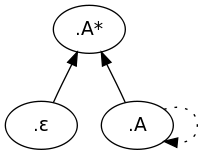
\includegraphics[scale=0.5]{star-list.png}
\caption{A graph representation of an expanded star-list; the solid arrows represent edges and the dotted arrows `next pointers' in the production.}
\end{figure}

These list children can be shared just like any other graph node. Nothing special needs to be done for this. Since this is the case, worst-case time and space bounds do not change by the introduction of this feature.

Exactly the same principle is used for separated lists and optionals. We will not go into detail on those, since one can easily imagine how these work.

\subsection{Location}

There are also specialized graph nodes for location related indicators. We have the following varieties:
\begin{enumerate}
 \setlength{\itemsep}{0pt}
 \setlength{\parskip}{0pt}
 \setlength{\parsep}{0pt}
 
 \item Start-of-line
 \item End-of-line
 \item At-column($X$); where $X$ indicates the column number
\end{enumerate}
Basically these are epsilons that only match when we are at a specific location in the input. So they do not consume input and act more like filters then anything else. They can be very useful when parsing for certain languages.

\section{Optimizations}
\label{chap:optimizations}

The basic algorithm is fairly straightforward and relatively simple to implement. The naïve implementation will respect worst-case cubic time and space bounds, however adaptations can be made to improve its overall efficiency.

\subsection{General}

\subsubsection{Matching}
A minor performance improvement can be made by matching on entire literals at once, instead of on induvidual characters. This decreases the amount of necessary graph nodes and thus reduces stack activity, offsetting the performance overhead being scannerless brings along completely. Note that, to ensure correct behaviour, the level at which each literal ends is the level in which it needs to be handled.

\subsubsection{Look-ahead}
A more obvious optimization is adding support for look-ahead restrictions. By adding simple checks to the (generated) parser code, we can prevent unnecessary work; if a certain alternative will never match, we do not need to expect it. This both improves performance and will make recognizing / parsing deterministic for LL(k) grammars. When the prefix-sharing optimization (see section \ref{sec:prefixSharing}) is enabled, this will also be the case for all grammars that fall within the LR(k) class.

\subsubsection{Breadth-first}
Finally we would like to note that (eventhough it is mandatory for the correctness of our algorithm, as discussed in section \ref{subsec:breadthFirstVsDepthFirst}) a breadth-first general parsing algorithm, or breadth-first implementation of a general parsing algorithm is generally more efficient then a depth-first version. The guarantee of being level synchronized can be exploited by the recognizer / parser, enabling the possibility of handling certain things more efficiently; this mainly has a positive effect on memory usage.

\subsection{Edge related}
\label{sec:edgeOptimizations}

Generally parsers store results on edges in the graph. If we would refrain from doing this and store parse results elsewhere (in a table with constant look-up time), edges could remain pointers. At first sight this may not look like an advantage, however we would be able to share edges among graph nodes and it opens up numereous other opportunities for optimization.

\subsubsection{Expansion}
\label{subsec:nodeExpansionOptimization}
First of all, by caching `expected children' for every type of node per level a substantial performance increase can be achieved. Additionally, this will ensure linear scaling for non-left-factored grammars. The reason for this is the following; for example, if we take the grammar rules:\\
$S\,::=\,E$\\
$E\,::=\,E + E\,|\,E - E$\\
The expansion at the first level would look like this:
\begin{enumerate}
 \setlength{\itemsep}{0pt}
 \setlength{\parskip}{0pt}
 \setlength{\parsep}{0pt}
 
 \item $.E$ $\rightarrow$ $.E+E$
 \item $.E+E$ edges = \{$.E$\}
 \item $.E$ $\rightarrow$ $.E-E$
 \item $.E-E$ edges = \{$.E$\}
 \item $.E+E$ $\rightarrow$ $.E+E$
 \item $.E+E$ edges = \{$.E$, $.E+E$\}
 \item $.E+E$ $\rightarrow$ $.E-E$
 \item $.E-E$ edges = \{$.E$, $.E+E$\}
 \item $.E-E$ $\rightarrow$ $.E+E$
 \item $.E+E$ edges = \{$.E$, $.E+E$, $.E-E$\}
 \item $.E-E$ $\rightarrow$ $.E-E$
 \item $.E-E$ edges = \{$.E$, $.E+E$, $.E-E$\}
\end{enumerate}
This example clearly demonstrates quardratic behaviour. If we would cache the edges set of one $E$, we could reuse it for any other $E$ in the same level and enable us to update it with additional edges by reference. This is possible since nodes are guaranteed to have the same edges if they are `expected' by the same parent(s). This will make the expansion look like this:
\begin{enumerate}
 \setlength{\itemsep}{0pt}
 \setlength{\parskip}{0pt}
 \setlength{\parsep}{0pt}
 
 \item $.E$ $\rightarrow$ $.E\,+\,E$
 \item $.E$ $\rightarrow$ $.E\,-\,E$
 \item $E$ edges = \{$.E$\}
 \item $.E+E$ $\Rightarrow$ $E$ edges += $.E+E$
 \item $.E-E$ $\Rightarrow$ $E$ edges += $.E-E$
\end{enumerate}
Now expansion completes in linear time. An additional benefit is that all the edge sets are shared between the children of the different $E$'s, saving memory. It will reduce the worst-case number of edges to $N\,*\,\mathit{numberOfSorts}$. Originally, without this kind of sharing, this would have been $N\,*\,\mathit{numberOfProductions}^2$, so this is a massive improvement. One other benefit of this optimization is that it lessens the need for the left-factoring of grammars. In absence of look-ahead filtering expansion performance should be on par with the non-factored equivalent of the grammar; in cases where look-ahead information is used, it may be close enough to remove its necessity.

Also note that this optimization is not only useful in case we have numereous non-factored productions. It also causes the set of edges to be shared between different alternatives associated with the same left-hand-side. So even if we would share the prefixes of all the alternatives (see \ref{sec:prefixSharing}), we would still gain something.

In section \ref{sec:factoringBenchmark} we look at some experimental results related to this optimization.

\subsubsection{Sharing}
Secondly, since the sets of edges, mentioned in section \ref{subsec:nodeExpansionOptimization}, are uniquely associated with a level and a certain non-terminal sort, we can reuse these sets of edges for each node in the production. When moving to the next node in a production we transfer each of the sets of edges to this next node, depending whether or not it is present yet; if a set of edges is present for a certain level in this next node, it is guaranteed to be the exact same set of edges as we are trying to add. Because of this guarantee, it will never be necessary to duplicate these sets or any of its content. So in any scenario the worst-case number of edges that will be constructed during a parse will never exceed $N\,*\,\mathit{numberOfSorts}$, or $O(N)$, in total. This is quite an improvement over the original ${N}^2\,*\,\mathit{numberOfProductions}^2$ we would have had without either of the edge sharing optimizations.

\subsubsection{Visiting}
\label{subsec:edgeVisitOptimization}
As mentioned before, since every graph node that contains the same non-terminal sort always has the same children if they are in the same level, it is sufficient to initially just follow the first edge in the edge set associated with that level. In case the node this edge points to has already been reduced, nothing needs to be done for this node or any of the other edges in this set (except record the results for the alternative, in case we are parsing and not just recognizing); otherwise all other edges in this set need to be followed as normally would have been the case, to queue their associated nodes for reduction. This reduces the number of edge visits significantly. Additionally, it enables us to quickly determine whether or not the parents of a node still need to be reduced or not, without having to execute any additional checks.

\subsection{Graph}

\subsubsection{Prefix sharing}
\label{sec:prefixSharing}
In many grammars productions exist that start with the same symbols. There is no reason to do duplicate work for these symbols. For example, if we take the grammar rule: $S\,::=\,E\,+\,E\,|\,E\,-\,E$. Both $E$'s at the start of these productions will always be derived exactly the same way for the same substring(s) and thus they are equal. Because of this, the prefixes of these two productions may as well be merged; i.e. by converting the rule into $S\,::=\,E\,(+\,E\,|\,-\,E)$. It is trivial to modify our algorithm to support this. Simply by allowing every node in the graph to have more then one `next' node and assigning the same id to both $E$'s (to indicate they must be shared), the desired result can be achieved. Naturally the merged prefixes of grammar rules can be arbitrarily long and are not restricted to just two partially equal rules; as long as the prefix for the rule overlaps with that of another rule, it can be merged, regardless whether or not it already has been merged with another rule.

This optimization ensures we can recognize and parse all types of LR grammars in linear time. The reason for this is that there will always be one active stack at most, thus each visit of a level completes in $O(1)$ time. This leads to the conclusion that the total recognize / parse time for any LR grammar will be $O(N)$, where $N$ is the length of the input.

One may wonder why merging anything other then the prefixes of productions is not supported. While in theory sharing the postfixes of production is also possible, this is more complicated to implement (for reasons we will not elaborate on here) and opportunities to apply this optimization rarely occur in reality. For these reasons we decided not to add this feature to our recognizer / parser. Merging blocks of symbols that are not located at either the beginning or end of productions will never be possible when using our algorithm, since this may lead to incorrect results. For example if we had shared the $B$ of the following alternatives: $S\,::=\,ABC\,|\,DBE$ we would also end up with derivations for $ABE$ and $DBC$, which is obviously undesirable.

\section{Filtering}
\label{chap:filtering}

As is common in general parsing, ultimately you often end up with an ambiguous parse forest. In this chapter we will discuss a number of features that can be used to filter the trees in this forest. These features are all optional and have no dependencies on eachother.

\subsection{Follow restrictions}

Follow restrictions work as a kind of disallowed look-ahead after the production; if the production we are trying to reduce matches the specified character(s) after the current location in the input, the reduce fails. They are mainly, though not exclusively, used to indicate eagerness.

Other variations are also possible. Like applying a similar restriction to preceding characters, or even the matched substring in its entirety.

\subsection{Rejects}

Reject filtering is intended for the removal of trees that are considered not to be correct at a certain location in the grammar. One could think of using it for things like filtering alternatives for identifiers that match keywords in the language, for example.

Any alternative of a production can be marked as reject. If this reject alternative matches, all other alternatives this reject belongs to are discarded. In our current implementation, rejected nodes are partially discarded at parse time and partially during post-parse filtering / flattening. Removing rejected stacks while parsing prevents unnecessary work from being performed; however it can be expensive to do in case reductions for the node associated with the rejected alternative were already performed, as we would need to transitively revisit all the outgoing edges and perform the necessary updates accordingly. This is the reason why it is not completely done at parse time.

In our current implementation reject rules cannot be nested, since this may lead to incorrect behaviour. Consider the following grammar: $S\,::=\,A(r)\,|\,a,\,A\,::=\,B(r)\,|\,a,\,B\,::=\,a$. The reject alternatives are marked with $(r)$. In this case the order in which reductions are done will determine the final parse result. For example, we could follow the edges from $.a$ to $.A$ and then from $.A(r)$ to $.S$. This will cause $S.$ to be rejected, failing the parse. On the other hand, if we would have followed the edge from $.a$ to $.B$ first and then from $.B(r)$ to $.A$ we would end up with a successful parse, since $A$ gets rejected, preventing the edge from $.A(r)$ to $.S$ from being followed. So if one writes a grammar that contains nested rejects it may, or may not do what was intended.

It is possible to resolve this problem, however this would require a second pass over the tree. Additionally it would prevent us from being able to remove parses that will be filtered in the end, before exploring them further. So it would impact performance in more then one way. This is the main reason why we decided not to support nested reject rules.

\subsection{Priorities and associativity}

Priorities and associativity restrictions are implemented as `don't nest' relations. For example, if we take the grammar rule $E\,::=\,E\,*\,E\,>\,E\,+\,E$, this means that the production $E\,+\,E$ cannot be a child of $E\,*\,E$ on either side of the production. $E\,::=\,E\,+\,E\,\{left\}$ on the other hand means that the production $E\,+\,E$ only cannot be a child of itself on the right hand side of the production; similarly for $\{right\}$, but the other way around. If declared as $\{nonassoc\}$ it cannot be nested on either side of itself.

The current implementation handles priority and associativity filtering completely at parse time. While reducing, it checks whether or not the reduction is allowed for the edge we want to follow; in case it is, it is stored in a result node that is identified by the sort name of the non-terminal of the node the edge points to and the set of `don't nest' relations associated with this node. This is because the result needs to be shared between all non-terminals with the same sort and `don't nest' relations. For example consider the following grammar rule: $E\,::=\,E * E\,\{left\}\,>\,(E + E\,|\,E - E)\{left\}$. Here the items $.E + E$ and $.E - E$ would be derived in the same way and thus should share their parse results, just as $E+.E$ and $E-.E$, since their `don't nest' relations are identical.

The main advantage of handling priority and associativity filtering at parse time oppossed to implementing it as post-parse filter is that it is more efficient. We prevent the construction of results that will be thrown away later on, saving memory. Additionally it will prevent unnecessarilly exploring certain parses, because we can determine they will be filtered earlier on, increasing performance. For certain grammars the benefits of this approach can be very significant. Furthermore, it also enables the possibility of constructing a recognizer for languages in which priorities and associativity are used for disambiguation (in absence of the application of filters that require a tree to be build).

There is a down-side however. Handling priority and associativity filtering at parse time, disables the edge visit reduction optimization discussed in section \ref{subsec:edgeVisitOptimization}, since we now always need to visit each of the outgoing edges of the node at every reduction to check whether or not the nesting is allowed. There is a tradeoff here and it will depend on the grammar whether or not the loss of this optimization can be compensated by what we gain by doing priority and associativity filtering at parse time, opposed to implementing it as a post-parse filter. In our opinion this should be the case for most `real' grammars.

\subsection{Actions}

Each grammar rule can have a number of actions associated with it. These actions can be used to filter alternatives that cannot be disambiguated using other filters, disambiguate non-context-free ambiguities (like C typedefs) or even influence the behaviour of the parser while it is running.

The option exists to either intergrate the execution of actions into the core of the parser itself or to apply them as a post-parse filter during, or after, flattening; depending on the requirements or preference of the user. However their implementation is not trivial, because of their interaction with ambiguities and the parse forest.

Unfortunately, we will not go into detail about this feature, since actions are outside of the scope of this article.

\section{Benchmarks}

In this chapter we will have a look at the performance of the current Java implementation of our algorithm.

Benchmarks were executed on a machine with the following specifications:
\begin{table}[H]
\centering
\begin{tabular}{ | p{6em} | p{9em} | }
 \hline
 CPU & Intel Q6600 \\
 Memory & 8 GB DDR-800 \\
 OS & Fedora Core 12 \\
 JRE & Sun 1.6.0\_13 (32-bit) \\
 JRE options & -Xmx1800m \\
 \hline
\end{tabular}
\end{table}

Measurements are listed in terms of CPU-time (system + user time) and are gathered using Java's build in management tool. Before performing the benchmarks, the recognizer / parser code was executed a number of times so Java's JIT compiler has the opportunity to optimize.

\subsection{Worst case}

The obvious candidates for a benchmark are the following worst-case grammars:
$S\,::=\,SSS\,|\,SS\,|\,a$\\
And:\\
$S\,::=\,SSS\,|\,SS\,|\,a\,|\,\epsilon$\\
With as input:\\
$a\,*\,50$ to $a\,*\,500$ at $50$ character intervals.

Note however that the recognizer is optimized for speed and the parser for a balance between memory usage and speed (meaning a faster implementation is possible at the cost of an increased memory footprint).

\begin{figure}[H]
\centering
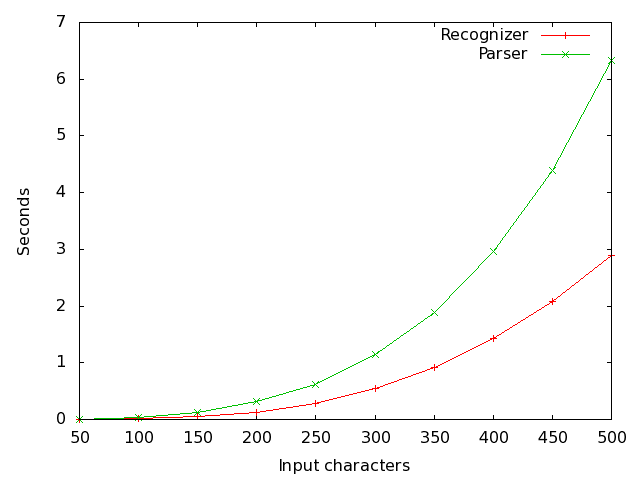
\includegraphics[scale=0.4]{worst-case.png}
\caption{$S\,::=\,SSS\,|\,SS\,|\,a$ recognizer and parser performance scaling.}
\end{figure}

\begin{figure}[H]
\centering
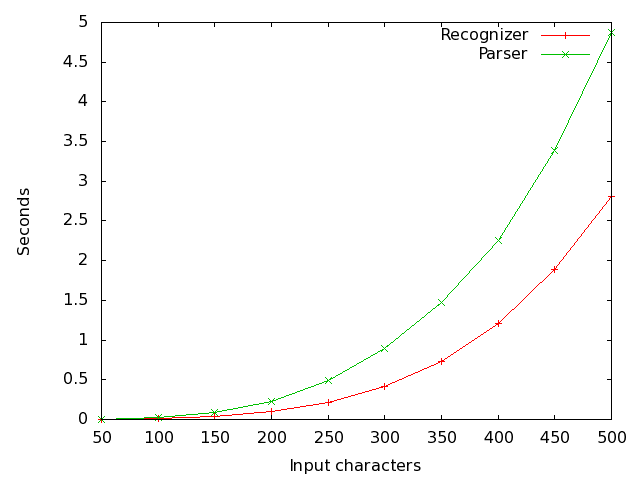
\includegraphics[scale=0.4]{worst-case_with-epsilon.png}
\caption{$S\,::=\,SSS\,|\,SS\,|\,a\,|\,\epsilon$ recognizer and parser performance scaling.}
\end{figure}

Our recognizer and parser implementations clearly demonstate cubic worst-case behaviour, as expected. Looking at the times, our implementation seems very efficient in worst-case scenarios.

What may appear surprising to some is the limited performance difference between both cases. Even though the version with the $\epsilon$ yields a more complicated tree and nullables need some special care, the actual extra work involved in handling them is negligable. This is in line with what we asserted in section \ref{subsec:hiddenRightRecursion}.

\subsection{Grammar factoring}
\label{sec:factoringBenchmark}

Apart from worst-case behaviour in terms of the number of ambiguous parse results, it is also interesting to look at how well we perform on a different kind of worst-case grammars, without ambiguous input. Here we will compare the performance of our parser between different version of a grammar; a non-factored non-prefix-shared version, a non-factored prefix-shared version and a left-factored version. The original grammar is the following:\\
$S\,::=\,E+$\\
$E\,::=\,a\,|\,E\,+\,E\,|\,E\,-\,E\,|\,E\,*\,E\,|\,E\,/\,E\,|\,E\,>\,E\,|\,...$ 25 more like it ...\\
Input = $a\,*\,50000$, $a\,*\,100000$, $a\,*\,150000$ and $a\,*\,200000$

It contains lots of recursion and is highly ambiguous; the input, on the other hand, can not be parsed in more then one way. Regardless, normally one would expect non-linear performance when parsing a string for this grammar. However, as can be seen in the graph below, this is not the case for our algorithm. In this benchmark, performance seems to scale perfectly linear regardless of how the grammar is factored.

\begin{figure}[H]
\centering
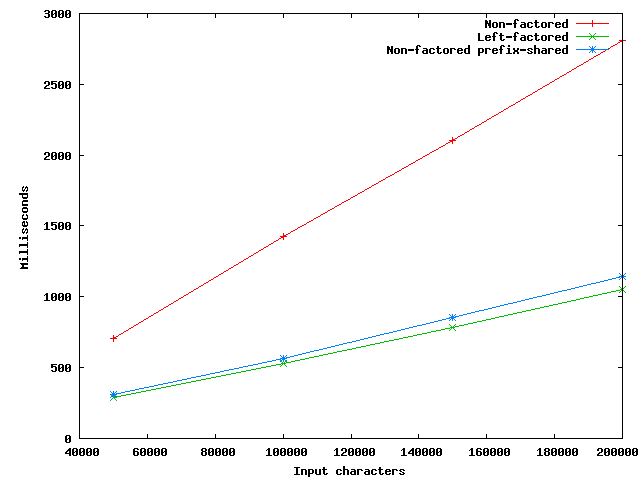
\includegraphics[scale=0.55]{grammar-factoring.png}
\caption{Grammar factoring related parse time scaling; without look-ahead filtering.}
\end{figure}

Note how the parser is more then twice as slow on the non-factored version of the grammar when prefix sharing is disabled. This is because both the number of graph nodes as the number of edge visits is significantly higher for this case. Regardless of this, parsing performance still scales linear with respect to the length of the input, due to the optimization discussed in section \ref{subsec:nodeExpansionOptimization}. This also supports the claims made in section \ref{subsec:unambiguousTimeComplexity}.

The non-factored prefix-shared and the left-factored versions of the grammar perform almost similar. The main reason that the parser using the left-factored version of the grammar performs slightly better is that our current implementation needs to do a little extra work to detect the sharing. However, if required, it is reasonably simple to construct an implementation of our parsing algorithm that does not suffer from this overhead. Additionally, left-factoring the grammar also removes all ambiguities from it. Counterary to what one might think, this does not have an impact on performance in this specific case. The reason for this is that look-ahead filtering was disabled for the purposes of this benchmark. If one would enable look-ahead filtering, parsing the left-factored version would become deterministic, since it falls within the LL(1) class of grammars.

\subsection{Versus non-general}

We also liked to know how we compare when pinned against non-general parsers, since general parsers have the image of being inferior in terms of performance, compared to `normal' LL or (LA)LR parsers.

We used the following basic LR grammar for our benchmark:\\
$S ::= E$\\
$E ::= E + F\,|\,F$\\
$F ::= a\,|\,(\,E\,)$\\
Input = `$A\,::=\,a\,|\,a+(A)$' from length $100003$, to length $1000003$ at $100000$ character intervals.

We compared our performance results with JavaCup, which was used in combination with JFlex. We selected JavaCup, since it is one of the more widely known and used parser generators that produce LALR parsers in Java.

\begin{figure}[H]
\centering
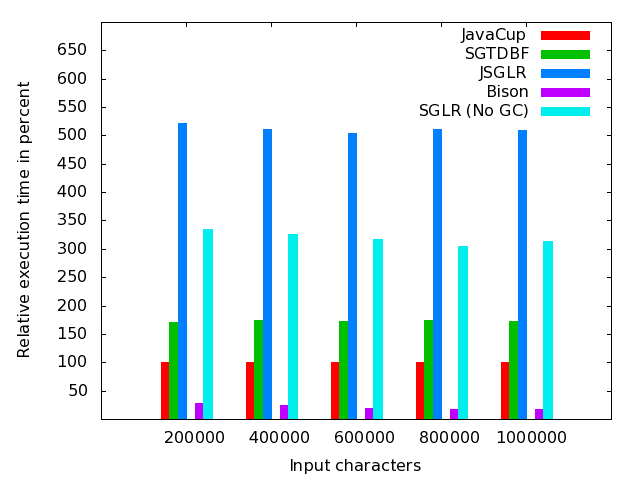
\includegraphics[scale=0.4]{vsLALR.png}
\caption{A parsing performance comparison with a LALR parser.}
\end{figure}

As expected JavaCup performs better. For this specific grammar, JavaCup consistently parses the given input somewhere between two and a half and three times as fast. This seems like a lot, however it is a fairly reasonable result. Especially considering we are using a graph, since we need to be fully general, instead of the application's stack.

\subsection{Realistic cases}

Benchmarks on artificial grammars are nice for getting a point across or to indicate certain guarantees can be met, however they generally do not offer any insight about performance in realistic cases. Here we will list a number of statistics related to parsing actual source files.

Note that, for now, we just list SDF2 files; a grammar definition format which is mildly ambiguous before filtering. In the future more results will be added for other languages.

\begin{table}[H]
\centering
\begin{tabular}{ | p{5em} | p{5em} | p{6em} | p{10em} |}
  \hline
  Filename & Input & Throughput & Throughput including\\
   & characters & (char/sec) & filtering \& flattening\\
   & & & (char/sec)\\
  \hline
  ATerm.def & 2393 & 341857 & 217545\\
  C.def & 10552 & 363862 & 245395\\
  SDF2.def & 18054 & 368448 & 234467\\
  Java.def & 30983 & 360267 & 232954\\
  \hline
\end{tabular}
\caption{Average parser throughput.}
\end{table}

One does have to take into account that our current implementation is written in Java. If we would re-implement it in C, a performance increase of at least three to five fold is to be expected. Putting our throughput at around 1 million characters per second, while having all filters enabled, in the SDF2 case.

Regardless of this, compared to the parser we previously used, a C implementation of scannerless GLR, we achieved a performance gain of roughly 40\% (i.e. our implementation parses the same file in 0.6 the amount of time), in this specific case.

\section{Prototype}

The development of this algorithm was approached in a rather unorthodox way. Rather then starting with the design of the algorithm and making an implementation for validation and testing purposes afterwards, we started with implementing a basic top-down recognizer, extending it to a parser, followed by testing, profiling and optimization; gradually we improved this implementation and its algorithm, until it matched our requirements. By using this type of approach we are able to get more direct feedback about issues and scalability and performance bottlenecks. Additionally, opportunities for optimization were highlighted that may not have been immediately apparent or which may have been overlooked when the problem would be approached from a purely algorithmic point of view.

The main purpose of this project has always been to create a working, usable general parser implementation. The development of a new algorithm was secondary but required, since no suitable alternative was available for our purposes.

Our first implementation is written in Java. The reason we chose this language for our prototype was that is was both required for our current project (the interpreter and IDE for the Rascal meta programming language), and gave us the opportunity to easily change and extend it. The down side is that it makes it harder to make a comparison with other general parser implementations, which are mainly written in C and consequently have a major performance advantage.

\section{Future work}

Numereous things can still be improved or changed. Mostly these involve optimizations or implementation improvements. We will not go into detail, but just list a number of ideas instead.

\begin{itemize}
 \setlength{\itemsep}{0pt}
 \setlength{\parskip}{0pt}
 \setlength{\parsep}{0pt}
 
 \item We can pre-construct a data structure which contains sort to alternatives mappings in combination with their look-ahead information, so we can obtain relevant alternatives more efficiently.
 \item Nullable derivations or trees can be pre-computed or dynamically cached, improving efficiency slightly.
 \item Matching could be handled more efficiently.
 \item Prefix sharing can be implemented more efficiently in our prototype, by moving more logic to the generator, so parts of productions do not have to be merged dynamically any more.
 \item Pre-computed information about priority / associativity restrictions can be used to handle filtering more efficiently.
 \item Multi-core / processor support is relatively easy to add and may be interesting to explore as possible performance booster for certain cases.
\end{itemize}

Finally, it would be interesting to create a C implementation of our parsing algorithm, both to see how far we can push the throughput of the parser and to be able to make a broader and more accurate performance comparison with implementations of other (general) parsing algorithms. We expect to do fairly well in such a showdown.

\section{Conclusion}

In this article we described our parsing algorithm, discussed optimizations that can be applied to it and gave an impression of its capabilities. To summarize, we developed a general parsing algorithm that is both easy to comprehend and scales and performs well, regardless of the input or grammar used. The best of both worlds, combined into one beautiful, elegant solution. Making compromises between performance and ease of use are now a thing of the past.

\pagebreak
\section{References}

TODO:\\
-GSS\\
-LL\\
-LR\\
-SPPF (and binarization)\\
-GLR\\
-SGLR (and ASF+SDF-Meta)\\
-JFlex\\
-JavaCup\\
-SDF2\\
-Rascal

\end{document}
